\documentclass{ti2}

% Dateikodierung ist utf8
\usepackage[utf8]{inputenc}   
\usepackage{graphicx}
\usepackage{listings}
\usepackage{rotating}
\usepackage{nonfloat}

\usepackage{wasysym}
\usepackage{dsfont}
\usepackage{enumitem}
%\usepackage{mathtools}

\lstset{
  numbers=left,
  numberstyle=\tiny,
  breaklines=true  
}

\begin{document}

% Nr, Abgabedatum, Gruppenleiter, Gruppenname, Name1...Name4
\Abgabeblatt{5}{05.12.2016}{Marc/Bingbin}{C05}%
                {Tabea Eggers}{Jan Fiedler}%
                {Florian Pflüger}{Jonas Schmutte}%

%\begin{listing}{1}
%\begin{listingcont}

\section*{Aufgabe 1}
\subsection*{a)}
Der Adressbereich von \emph{main}:\\
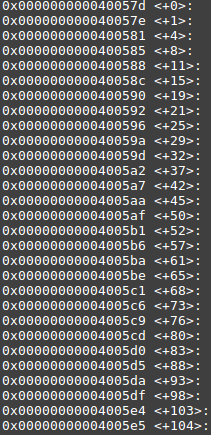
\includegraphics{aufgabe01/main.png}\\

Der Adressbereich von \emph{factorial}:\\
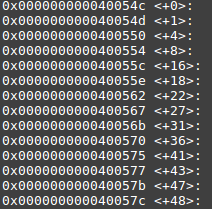
\includegraphics{aufgabe01/factorial.png}\\
Dabei ist zu beachten, dass sich eine Adresse x, deren Nachfolgeradresse y nicht x+1 entspricht, "uber die Gr"o"se von y-x Adressen ausdehnt.\\ 
\subsection*{b)}
Im Stacksegment wird auf die Adressen 0x7fffffffdf50 und 0x7fffffffdf40 zugegriffen.\\

Unser L"osungsweg:\\
Schritt f"ur Schritt durch \emph{factorial} debuggen und regelm"a"sig schauen, was in den Registern steht.\\
Bei Eintritt steht 0x7fffffffe668 in \emph{\%rsp.} 
Kurz vor dem mv-Befehl steht 0x7fffffffe660 in \emph{\%rsp}. Es wurde also -0x8 gerechnet.\\
Dies wird dann in \%rbp geschrieben.\\
Diese Werte ver"andern sich nun nicht mehr.\\
Es wird dann auf die Adressen -0x8(\%rbp) und -0x18(\%rbp) zugegriffen.
Das Entspricht 0x7fffffffe658 und 0x7fffffffe648.\\


Bildet man diesen Vorgang mit 0x7fffffffdf60 als \emph{\%rsp} Startwert, kommt man auf Zugriffe auf die Adressen 0x7fffffffdf50 und 0x7fffffffdf40,\\
\section*{c)}
Der von \emph{printf} in \emph{main} gelesene Format-String beginnt an 0x7fffffffe590. Diese Adresse wird in \_\_printf errechnet und in \%rsp gespeichert.\\
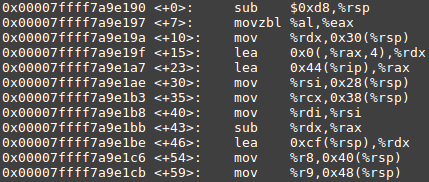
\includegraphics{aufgabe01/a1.png}

Es wird dann noch im zusammenhang mit dieser Zeichenkette auf die Adressen
0x7fffffffe5c0 (0x30(\%rsp)), 0x7fffffffe5b8 (0x28(\%rsp)), 0x7fffffffe5c8 (0x38(\%rsp)), 0x7fffffffe5d0 (0x40(\%rsp)) und 0x7fffffffe5d8 (0x48(\%rsp)) zugegriffen.  
 
\section*{d)}
Beispielrechnung f"ur 0x40057d:\\
Pagegr"o"se ist 4KiB also 4096B = 0x1000.\\
Die Page 0 startet beim Offset 0x1000000.\\
$Page: floor(0x40057d/0x1000) = 0x400 = 1024 \Rightarrow PF = 17363 = 0x43d3\\$
$Off: 0x40057d \% 0x1000 = 0x57d\\$
$Phys.Adresse: 0x43d3 * 0x1000 + 0x57d + 0x1000000 = 0x53d357d \\$ 

Mit gleicher Rechnung ergibt sich f"ur die Adressen aus \emph{main}\\
$0x40057e \Rightarrow 0x53d357e$\\  
$0x400581 \Rightarrow 0x53d3581$\\
$0x400585 \Rightarrow 0x53d3585 $\\
$0x400588 \Rightarrow 0x53d3588 $\\
$0x40058c \Rightarrow 0x53d358c $\\
$0x400590 \Rightarrow 0x53d3590 $\\
$0x400592 \Rightarrow 0x53d3592 $\\
$0x400596 \Rightarrow 0x53d3596 $\\
$0x40059a \Rightarrow 0x53d359a $\\
$0x40059d \Rightarrow 0x53d359d $\\
$0x4005a2 \Rightarrow 0x53d35a2 $\\
$0x4005a7 \Rightarrow 0x53d35a7 $\\
$0x4005aa \Rightarrow 0x53d35aa $\\
$0x4005af \Rightarrow 0x53d35af $\\
$0x4005b1 \Rightarrow 0x53d35b1 $\\
$0x4005b6 \Rightarrow 0x53d35b6 $\\
$0x4005ba \Rightarrow 0x53d35ba $\\
$0x4005be \Rightarrow 0x53d35be $\\
$0x4005c1 \Rightarrow 0x53d35c1 $\\
$0x4005c6 \Rightarrow 0x53d35c6 $\\
$0x4005c9 \Rightarrow 0x53d35c9 $\\
$0x4005cd \Rightarrow 0x53d35cd $\\
$0x4005d0 \Rightarrow 0x53d35d0 $\\
$0x4005d5 \Rightarrow 0x53d35d5 $\\
$0x4005da \Rightarrow 0x53d35da $\\
$0x4005df \Rightarrow 0x53d35df $\\
$0x4005e4 \Rightarrow 0x53d35e4 $\\
$0x4005e5 \Rightarrow 0x53d35e5 $\\

F"ur die aus \emph{factorial}:\\
$0x40054c \Rightarrow 0x53d354c$\\
$0x40054d \Rightarrow 0x53d354d$\\
$0x400550 \Rightarrow 0x53d3550$\\
$0x400554 \Rightarrow 0x53d3554$\\
$0x40055c \Rightarrow 0x53d355c$\\
$0x40055e \Rightarrow 0x53d355e$\\
$0x400562 \Rightarrow 0x53d3562$\\
$0x400567 \Rightarrow 0x53d3567$\\
$0x40056b \Rightarrow 0x53d356b$\\
$0x400570 \Rightarrow 0x53d3570$\\
$0x400575 \Rightarrow 0x53d3575$\\
$0x400577 \Rightarrow 0x53d3577$\\
$0x40057b \Rightarrow 0x53d357b$\\
$0x40057c \Rightarrow 0x53d357c$\\

F"ur die Adressen aus b:\\
Hier haben wir pagenummer 4294967293 gew"ahlt, da $Page(0x7fffffffdf50)= 0x7fffffffd = 34359738365$ nicht im Hauptspeicher ist. \\
Daher pageframe = 2001 = 0x7d1\\

$0x7fffffffdf50 \Rightarrow 0x7d1 * 0x1000 + f50 + 0x1000000 = 0x17d1f50 $\\
$0x7fffffffdf40 \Rightarrow 0x17d1f40$\\

F"ur Adressen aus c:\\
Hier haben wir pagenummer 4195813 gew"ahlt, da $Page(0x7fffffffe590)= 0x7fffffffe = 34359738366$ nicht im Hauptspeicher ist. \\
Daher pageframe = 100 = 64\
\
$0x7fffffffe590 \Rightarrow 0x64 * 0x1000 + 0x590 + 0x1000000 = 0x1064590 $\\
$0x7fffffffe5c0 \Rightarrow 0x10645c0 $\\
$0x7fffffffe5b8 \Rightarrow 0x10645b8 $\\
$0x7fffffffe5c8 \Rightarrow 0x10645c8 $\\
$0x7fffffffe5d0 \Rightarrow 0x10645d0 $\\
$0x7fffffffe5d8 \Rightarrow 0x10645d8 $\\



\newpage
\section*{Aufgabe 2}
Bei dieser Aufgabe haben wir mit der Gruppe \texttt{G05} zusammen gearbeitet.

Datei: 33696325 B \\
Datenblockgröße: 512 B \\
Berechnung der benötigten Datenblöcke: $33696325 : 512 = 65813,1347... \rightarrow 65814$ Datenblöcke, da aufgerundet werden muss (sonst fehlen Daten) \\\\
Ein Indirektblock fasst 512 B. \\
Eine Datenblocknummer besteht aus 4 B. \\
Berechnung der möglichen Einträge in einem Indirektblock: $512 : 4 = 128$ Einträge \\\\
Eine Inode (= 1 Block) hat: \\
10 direkte Verweise \\
1 einfachen Indirektblock \\
1 doppelten Indirektblock \\
1 dreifachen Indirektblock \\\\
\begin{tabular}[h]{|c|c|c|}
	\hline
	 & Anzahl der Verweise auf Datenblöcke & benötigte Indirektblöcke \\
	\hline
	\hline
	einfacher Indirektblock & 128 & 1 \\
	\hline
	doppelter Indirektblock & $128^2 = 16384$ & $1 + 128$ \\
	\hline
	dreifacher Indirektblock & $128^3 = 2097152$ & $1 + 128 + 128^2$ \\
	\hline
\end{tabular} \\\\
einfacher + doppelter Indirektblock : 16502 mögliche Verweise \\
Berechnung der noch fehlenden Verweise: $65804 ~\textit{(Da in der Inode schon 10 Direktverweise sind) } - 16502 = 49302$ fehlende Einträge \\
Da die mögliche Anzahl von Verweisen beim dreifachen Indirektblock mehr als ausreichend ist, rechnet man: \\
$49302 : 128 ~\textit{(Anzahl der Einträge die ein Datenblock enthalten kann)} = 385,1718... \rightarrow 386$ noch benötigte Indirektblöcke der dritten "'Ebene" (auch hier aufrunden)\\
um nun die zweite "'Ebene" zu bekommen rechnet man: $386 : 128 = 3,0156... \rightarrow$ 4 Indirektblöcke in der zweiten "'Ebene", wovon einer nicht vollständig ausgenutzt wird \\
Man erhält also für den dreifachen Indirektblock: \\
$\underbrace{1}_{\shortstack{Indirektblock\\ der ersten Ebene}} + \underbrace{(3 + 3 \cdot 128)}_{\shortstack{Indirektblock\\ der zweiten Ebene}} + \underbrace{(1 + 2)}_{\shortstack{Indirektblock der\\ dritten Ebene mit\\ Block aus zweiter\\ Ebene der auf\\ Block in dritter\\ Ebene verweist}}  = ~391$ benötigte Indirektblöcke \\\\
Nun lässt sich die Zahl der insgesamt benötigten Datenblöcke für die Datei berechnen: \\
65814 Datenblöcke (durch die Datei) \\
+ 1 Block (Inode) \\
+ 1 Indirektblock (einfacher Indirektblock) \\
+ 129 Indirektblöcke (doppelter Indirektblock) \\
+ 391 Indirektblöcke (dreifacher Indirektblock) \\
-------------------------------------------------------------- \\
66336 Blöcke braucht man für die Datei insgesamt.



\section*{Aufgabe 3}
Bei dieser Aufgabe haben wir mit der Gruppe \texttt{F02} zusammen gearbeitet.

\emph{open( ``/home/ti2/archive/nikolaus.avi'', O\_RDONLY );}

\begin{itemize}
	\item Inode (0, /) ist in der Inode-Tabelle
	\item Datenblock von Inode 0 ist im Buffer-Cache
	\item Da Inode 0 ein Verzeichnis ist, steht da eine Tabelle mit den
	Dateinamen und den dazu gehörigen Inode-Nummern drin, welche in
	\emph{/} sind. Diese Tabelle durchsuchen wir nach \emph{home}.
	\item \emph{home} hat die Inode-Nummer 36
	\item Inode 36, in die Inode-Tabelle eintragen und den dazugehörigen
	Datenblock 9 in den Cache laden.
	\item Da \emph{home} ein Verzeichnis ist, haben wir also wieder eine Tabelle
	mit den nächsten Komponenten und deren Inode-Nummern. Suchen nach
	\emph{ti2}
	\item \emph{ti2} hat die Nummer 99.
	\item Also in die Inode-Tabelle eintragen und den Datenblock 2000 in den
	Cache laden
	\item \emph{ti2} ist ein Verzeichnis welches wir dann nach den Eintrag
	\emph{archive} durchsuchen. \emph{archive} hat Inode-Nummer 206.
	\item Inode 206 eintragen und den Datenblock 3101 in den Cache holen
	\item Die Tabelle von \emph{archive} nach \emph{nikolaus.avi} durchsuchen,
	da \emph{archive} ein Verzeichnis ist
	\item \emph{nikolaus.avi} hat die Inode-Nummer 12783
	\item Inode in die Tabelle eintragen
	\item Nun kann der FileDiscriptor zurückgegeben werden, weil wir das Ziel
	erreicht haben
	(Es kann noch sein das die Datei schon geladen wird, auf den Verdacht hin das gleich auf diese zu gegriffen wird)
\end{itemize}

\emph{open( ``/home/ti2/meta'', O\_RDWR );}

\begin{itemize}
	\item Das gleiche Spiel wie eben durch die Inodes von \emph{/} und
	\emph{home} zu \emph{ti2} navigieren, bloss befinden sich die Inodes
	schon in der Tabelle und die Datenblöcke im Cache.
	\item Den Datenblock von \emph{ti2} durchsuchen wir nun nach \emph{meta}
	\item \emph{meta} hat die Inode-Nummer 112
	\item Die Inode tragen wir in die Tabelle ein
	\item Danach wird der FileDiscriptor zurückgegeben
\end{itemize}

\emph{lseek( f, -10000, SEEK\_END);}

\begin{itemize}
	\item Schieb den FileDiscriptor an das 10000 vorletzte Byte von der
	\emph{Nikolaus.avi}
\end{itemize}

\emph{read( f, buf, 4096 );}

\begin{itemize}
	\item Liest 4096 Bytes aus den passenden Datenblöcke der \emph{nikolaus.avi}
	und schreibt diese in \emph{buf}
	\item und gibt die Anzahl der tatsächlich gelesenden Bytes zurück
\end{itemize}

\emph{write( g, buf, count );}

\begin{itemize}
	\item Nun werden die Bytes in \emph{meta} geschrieben
	\item Danach werden die Metadaten in der Inode aktualisiert
\end{itemize}

\end{document}
